\documentclass[12pt,a4paper]{article}

% ------------------------------------------------------------------
% Packages
% ------------------------------------------------------------------
\usepackage[utf8]{inputenc}
\usepackage[T1]{fontenc}
\usepackage[english]{babel}
\usepackage[a4paper,top=2.5cm,bottom=2.5cm,left=3cm,right=2.5cm]{geometry}
\usepackage{amsmath}
\usepackage{amssymb}
\usepackage{graphicx}
\usepackage{booktabs}
\usepackage{siunitx}
\usepackage{caption}
\usepackage{subcaption}
\usepackage{float}
\usepackage{setspace}
\usepackage[hidelinks]{hyperref}

\sisetup{detect-weight=true,detect-family=true}
\DeclareSIUnit{\atm}{atm}
\onehalfspacing
\graphicspath{{figures/}}

\captionsetup{font=small,labelfont=bf}

% Chemistry shortcuts
\newcommand{\NHH}{NH\textsubscript{3}}
\newcommand{\HH}{H\textsubscript{2}}
\newcommand{\OO}{O\textsubscript{2}}
\newcommand{\NN}{N\textsubscript{2}}
\newcommand{\NO}{NO}
\newcommand{\NOx}{NO\textsubscript{x}}
\newcommand{\NOO}{NO\textsubscript{2}}
\newcommand{\NNO}{N\textsubscript{2}O}
\newcommand{\SL}{$S_\mathrm{L}$}
\newcommand{\phieq}{\varphi}
\newcommand{\XH}{$X_{\HH}$}

% ------------------------------------------------------------------
\begin{document}

% ============ TITLE PAGE ============
\begin{titlepage}
\centering
\vspace*{1.5cm}
{\scshape\large Warsaw University of Technology\par}
{\scshape Faculty of Power and Aeronautical Engineering (MEiL)\par}
\vspace{0.5cm}
{\large Computational Methods in Combustion (MKWS)\par}
\vfill
{\Huge\bfseries Laminar Flame Speed and \NOx{} Formation in Ammonia--Hydrogen--Air Blends\par}
\vspace{0.8cm}
{\large Effect of hydrogen enrichment, equivalence ratio and preheat temperature\par}
\vfill
\begin{flushright}
\large
Author: Antoni Balcy (album no.\ 333439)\\[0.2cm]
Supervisor: mgr inż.\ Mateusz Żbikowski\\[0.2cm]
\end{flushright}
\vspace{1cm}
{\large Academic year 2025/2026\par}
\end{titlepage}

\tableofcontents
\newpage

% ============ 1. INTRODUCTION ============
\section{Introduction}

Ammonia (\NHH) has attracted strong renewed interest as a carbon-free fuel and
as a practical hydrogen carrier: it contains no carbon, liquefies under mild
pressure, and benefits from an existing global production and transport
infrastructure. Its direct use in combustion systems is, however, hampered by
two well-known drawbacks. First, ammonia burns very slowly --- its laminar
flame speed \SL{} at stoichiometric, atmospheric conditions is only about
\SI{6}{\centi\meter\per\second}, roughly one fifth of that of methane. This
makes flame stabilisation difficult and narrows the operating envelope.
Second, because ammonia carries fuel-bound nitrogen, it is prone to high
nitrogen-oxide (\NOx{}) emissions.

A widely studied remedy is to blend ammonia with hydrogen (\HH). Hydrogen has
an extremely high reactivity and flame speed, so even modest additions
substantially accelerate the ammonia flame. The price of this improvement is
typically a higher flame temperature and, with it, a tendency toward increased
thermal \NOx{}. The fuel therefore presents an intrinsic
\emph{flame-speed versus \NOx{} trade-off} whose shape depends on the blend
composition, the mixture stoichiometry and the operating temperature.

The aim of this project is to characterise that trade-off quantitatively using
one-dimensional laminar flame simulations in Cantera. Three control variables
are swept: the hydrogen mole fraction in the fuel \XH{}, the equivalence ratio
$\phieq$, and the unburned-mixture (preheat) temperature $T_\mathrm{in}$. The
results are summarised as contour maps of \SL{} and \NOx{}, as an explicit
Pareto front of the trade-off, and as an analysis of the preheat effect. The
study identifies operating regions that combine an acceptable flame speed with
a substantially reduced \NOx{} output.

% ============ 2. LITERATURE / BACKGROUND ============
\section{Theoretical Background}

\subsection{Laminar flame speed}
The laminar flame speed \SL{} is the velocity at which a planar,
one-dimensional, premixed flame front propagates into a quiescent unburned
mixture, measured relative to the unburned gas. It is a fundamental property of
a fuel--oxidiser mixture that depends on chemical kinetics, thermodynamics and
molecular transport. In a freely propagating flame the mass burning rate
$\dot{m}=\rho_\mathrm{u} S_\mathrm{L}$ is an eigenvalue of the governing
conservation equations and is obtained directly from the converged solution.

\subsection{\NOx{} formation}
Nitrogen oxides form through several coupled routes. In hydrocarbon and
hydrogen flames the \emph{thermal} (Zeldovich) mechanism dominates: it is
strongly temperature-activated and therefore grows rapidly once the flame
temperature exceeds roughly \SI{1800}{\kelvin}. In ammonia combustion an
additional \emph{fuel} \NOx{} route is important, because nitrogen released from
the fuel is partly oxidised to \NO{} via amine ($\mathrm{NH}_i$) intermediates.
The net \NOx{} therefore reflects a balance between formation (favoured by high
temperature and excess oxygen) and reduction (favoured by fuel-rich conditions,
where \NO{} is consumed by $\mathrm{NH}_i$ radicals --- the basis of the
``\NHH{}-deNOx'' / SNCR effect). In this work \NOx{} is reported as the sum of
\NO{} and \NOO{} mole fractions in the burned gas.

\subsection{Equivalence ratio and preheat}
The equivalence ratio $\phieq$ measures the fuel-to-oxidiser ratio relative to
stoichiometric: $\phieq<1$ is lean, $\phieq>1$ is rich. Both \SL{} and the
flame temperature usually peak slightly rich of stoichiometric. Preheating the
unburned mixture raises the flame temperature and accelerates the kinetics,
increasing \SL{} markedly, but it also tends to raise thermal \NOx{}.

% ============ 3. MODEL ============
\section{Numerical Model}

\subsection{Configuration}
The simulations use the one-dimensional freely propagating premixed flame model
\texttt{FreeFlame} of the open-source chemical-kinetics library Cantera
(version 3.2). The flame is solved on an adaptively refined grid; mixture-%
averaged transport is used as a balanced compromise between accuracy and
computational cost. All cases are computed at a pressure of \SI{1}{\atm}. Air is
represented with the molar composition \OO{}:1, \NN{}:3.76.

The chemistry is described by the GRI-Mech~3.0 mechanism
(\texttt{gri30.yaml}, 53 species, 325 reactions), which includes ammonia,
hydrogen and a complete nitrogen sub-mechanism (\NO{}, \NOO{}, \NNO{}). The fuel
is a binary \NHH{}/\HH{} blend characterised by the hydrogen mole fraction
\begin{equation}
X_{\HH} = \frac{n_{\HH}}{n_{\HH} + n_{\NHH}}.
\end{equation}

\subsection{Control variables}
Three parameters are swept independently, giving a total of $4\times7\times3=84$
converged flames:
\begin{itemize}
  \item Hydrogen fraction in fuel: $X_{\HH}\in\{0.0,\,0.2,\,0.4,\,0.6\}$;
  \item Equivalence ratio: $\phieq\in\{0.7,\,0.8,\,0.9,\,1.0,\,1.1,\,1.2,\,1.3\}$;
  \item Preheat temperature: $T_\mathrm{in}\in\{300,\,450,\,600\}~\si{\kelvin}$.
\end{itemize}

\subsection{Solution strategy and post-processing}
A \emph{continuation} strategy is used: within each $\phieq$ sweep, the
converged solution of the previous case is supplied as the initial guess for the
next. This significantly accelerates the sweep and improves robustness near the
lean and rich flammability limits. For each converged flame the following
scalars are extracted: the laminar flame speed \SL{} (the unburned-side flow
velocity), the adiabatic flame temperature $T_\mathrm{ad}$ (burned-gas
temperature), and the exhaust mole fractions of \NO{}, \NOO{} and \NNO{}. The
quantity \NOx{} is defined as
\begin{equation}
\mathrm{\NOx} = X_{\NO} + X_{\NOO},
\end{equation}
expressed in parts per million (ppm). All results are written to a CSV file and
processed with NumPy, pandas and Matplotlib.

% ============ 4. RESULTS ============
\section{Results and Discussion}

\subsection{Flame structure}
Figure~\ref{fig:profile} shows the internal structure of a representative flame
($X_{\HH}=0.4$, $\phieq=1.0$, $T_\mathrm{in}=\SI{300}{\kelvin}$). The temperature
rises sharply across a thin reaction zone while the fuel species \NHH{} and \HH{}
are consumed; \NO{} and the radical \mbox{OH} are produced in and just behind the
front. This confirms that the model captures both the heat-release structure and
the nitrogen chemistry needed for the present study.

\begin{figure}[H]
  \centering
  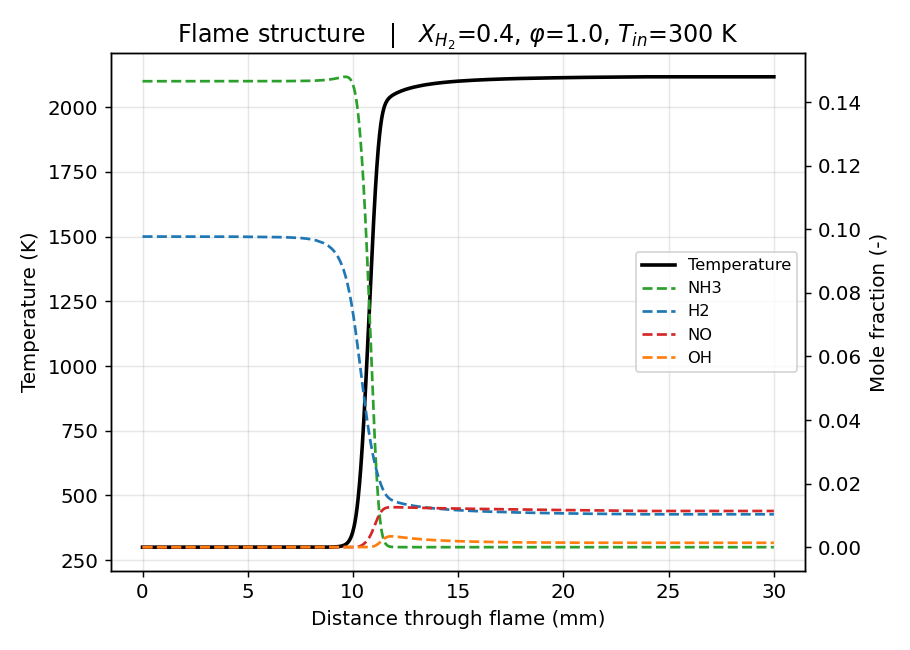
\includegraphics[width=0.78\textwidth]{fig6_flame_profile.png}
  \caption{Resolved flame structure: temperature (left axis) and selected species
  mole fractions (right axis) through the flame, for $X_{\HH}=0.4$, $\phieq=1.0$,
  $T_\mathrm{in}=\SI{300}{\kelvin}$.}
  \label{fig:profile}
\end{figure}

\subsection{Effect of hydrogen enrichment on flame speed}
Figure~\ref{fig:slxh2} shows the laminar flame speed as a function of \XH{} for
several equivalence ratios at $T_\mathrm{in}=\SI{300}{\kelvin}$, and
Figure~\ref{fig:slcontour} presents the same data as a contour map on the
$(\phieq,X_{\HH})$ plane. Hydrogen addition has a strong, strongly non-linear
effect. At stoichiometric conditions \SL{} rises from
\SI{5.9}{\centi\meter\per\second} for pure ammonia to
\SI{48.3}{\centi\meter\per\second} at $X_{\HH}=0.6$ --- an eight-fold increase.
The flame speed peaks consistently near $\phieq\approx1.1$, slightly rich of
stoichiometric, as expected. Table~\ref{tab:peaks} lists the peak flame speed
for each blend.

\begin{figure}[H]
  \centering
  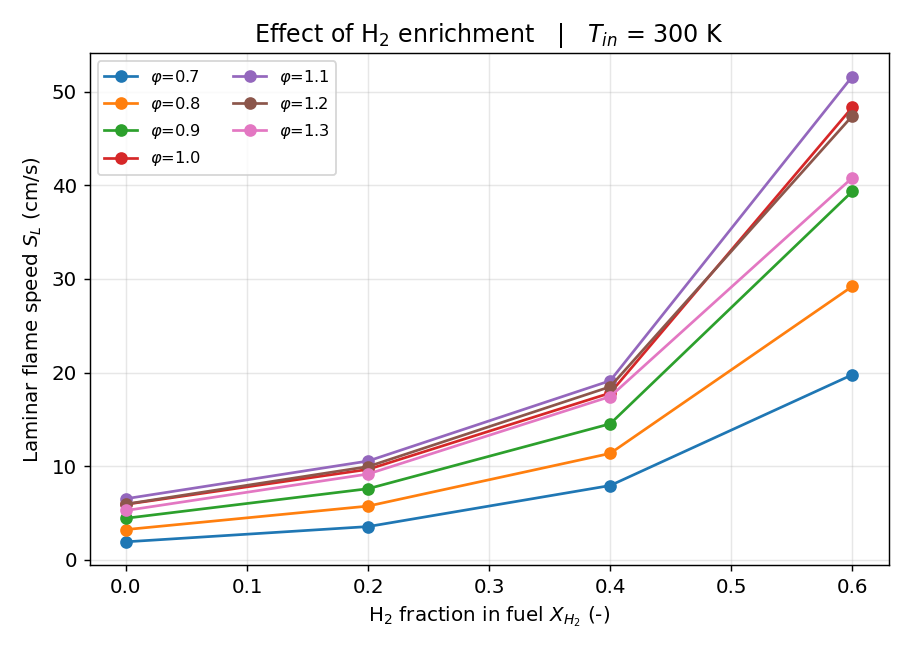
\includegraphics[width=0.80\textwidth]{fig3_SL_vs_XH2.png}
  \caption{Laminar flame speed versus hydrogen fraction in the fuel, for several
  equivalence ratios ($T_\mathrm{in}=\SI{300}{\kelvin}$, $p=\SI{1}{\atm}$).}
  \label{fig:slxh2}
\end{figure}

\begin{figure}[H]
  \centering
  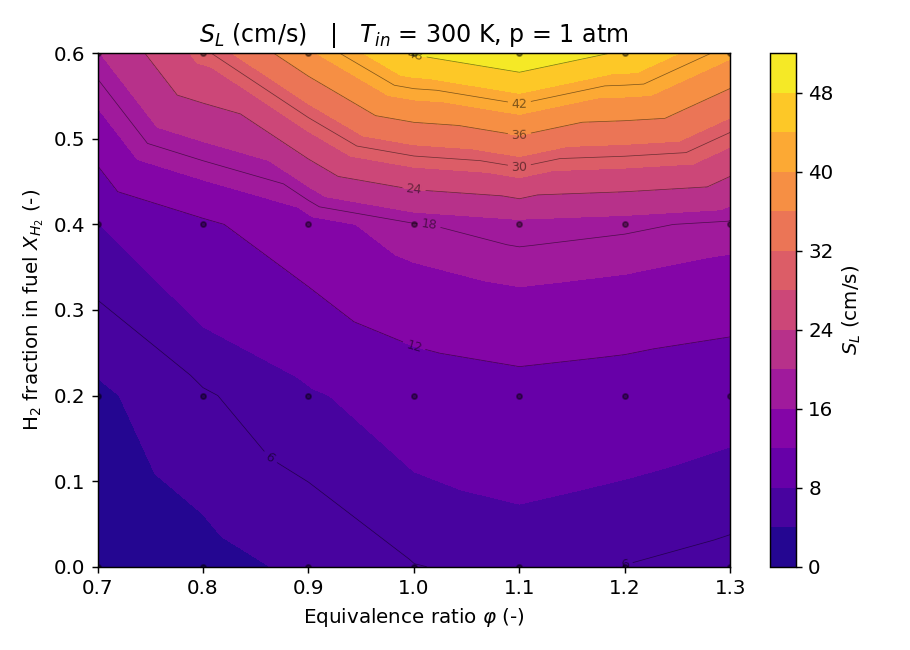
\includegraphics[width=0.78\textwidth]{fig1_SL_contour.png}
  \caption{Contour map of laminar flame speed \SL{} (\si{\centi\meter\per\second})
  on the $(\phieq,X_{\HH})$ plane at $T_\mathrm{in}=\SI{300}{\kelvin}$.}
  \label{fig:slcontour}
\end{figure}

\begin{table}[H]
  \centering
  \caption{Peak laminar flame speed and the corresponding \NOx{} for each blend
  ($T_\mathrm{in}=\SI{300}{\kelvin}$). The peak occurs at $\phieq=1.1$ in all cases.}
  \label{tab:peaks}
  \begin{tabular}{cccc}
    \toprule
    $X_{\HH}$ & $S_\mathrm{L}$ [\si{\centi\meter\per\second}] &
    $T_\mathrm{ad}$ [\si{\kelvin}] & \NOx{} [ppm] \\
    \midrule
    0.0 & 6.5  & 2007 & 2084  \\
    0.2 & 10.6 & 2041 & 4676  \\
    0.4 & 19.1 & 2103 & 5354  \\
    0.6 & 51.6 & 2139 & 10391 \\
    \bottomrule
  \end{tabular}
\end{table}

\subsection{\NOx{} emission}
Figure~\ref{fig:noxcontour} maps the exhaust \NOx{} over the same plane. Two
trends stand out. First, \NOx{} peaks on the lean side, between
$\phieq\approx0.8$ and $0.9$, where both flame temperature and oxygen
availability are high; the peak shifts slightly leaner as hydrogen is added.
Second, \NOx{} falls steeply as the mixture becomes rich: at $X_{\HH}=0$ it
drops from about \SI{11600}{ppm} at $\phieq=0.9$ to below \SI{1400}{ppm} at
$\phieq=1.2$, reflecting the consumption of \NO{} by amine radicals under
fuel-rich conditions. Increasing the hydrogen content raises \NOx{} overall,
consistent with the higher flame temperatures it produces.

\begin{figure}[H]
  \centering
  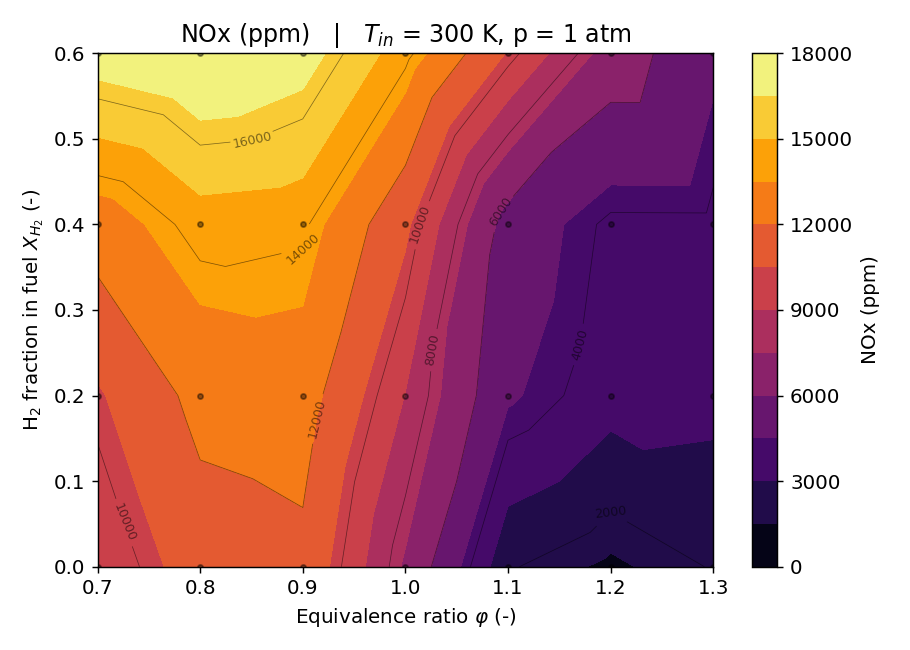
\includegraphics[width=0.78\textwidth]{fig2_NOx_contour.png}
  \caption{Contour map of exhaust \NOx{} (ppm) on the $(\phieq,X_{\HH})$ plane at
  $T_\mathrm{in}=\SI{300}{\kelvin}$.}
  \label{fig:noxcontour}
\end{figure}

\subsection{The flame-speed / \NOx{} trade-off}
The competing influences of \XH{} and $\phieq$ are summarised in the Pareto
diagram of Figure~\ref{fig:pareto}, which plots \NOx{} against \SL{} with points
coloured by equivalence ratio. The dashed Pareto front connects the operating
points that are not dominated --- those for which no other case offers both a
higher flame speed and a lower \NOx{}. The front is populated almost entirely by
fuel-rich points ($\phieq\approx1.2$--$1.3$, the yellow markers): mildly rich
operation retains most of the flame-speed benefit of hydrogen enrichment while
cutting \NOx{} by a large margin relative to the lean and stoichiometric cases.
This is the central practical result of the study.

\begin{figure}[H]
  \centering
  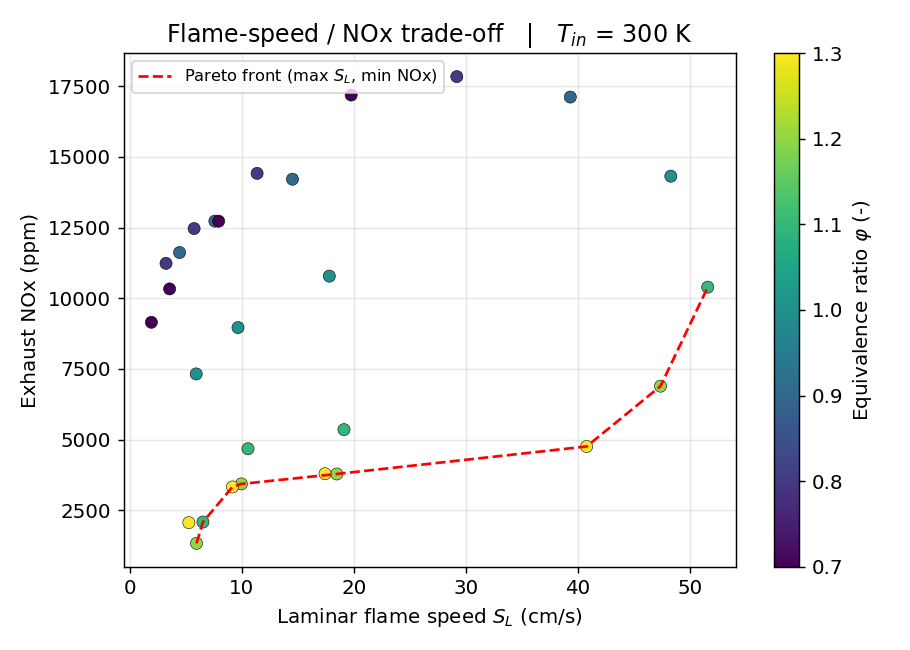
\includegraphics[width=0.80\textwidth]{fig4_pareto.png}
  \caption{Flame-speed / \NOx{} trade-off at $T_\mathrm{in}=\SI{300}{\kelvin}$.
  Points are coloured by equivalence ratio; the dashed line is the Pareto front
  (maximum \SL{}, minimum \NOx{}).}
  \label{fig:pareto}
\end{figure}

\subsection{Effect of preheat temperature}
Figure~\ref{fig:preheat} shows how preheating the unburned mixture affects \SL{}
and \NOx{} at a fixed operating point ($X_{\HH}=0.4$, $\phieq=1.0$). The effect on
flame speed is dramatic: \SL{} grows from \SI{17.8}{\centi\meter\per\second} at
\SI{300}{\kelvin} to \SI{71.4}{\centi\meter\per\second} at \SI{600}{\kelvin}, a
roughly four-fold increase. The accompanying rise in \NOx{} is comparatively
modest (from about \num{10800} to \SI{13800}{ppm}), because the increase in
flame temperature ($\approx\SI{170}{\kelvin}$) is moderate. Preheating is
therefore an effective lever for compensating ammonia's low reactivity at a
limited \NOx{} penalty.

\begin{figure}[H]
  \centering
  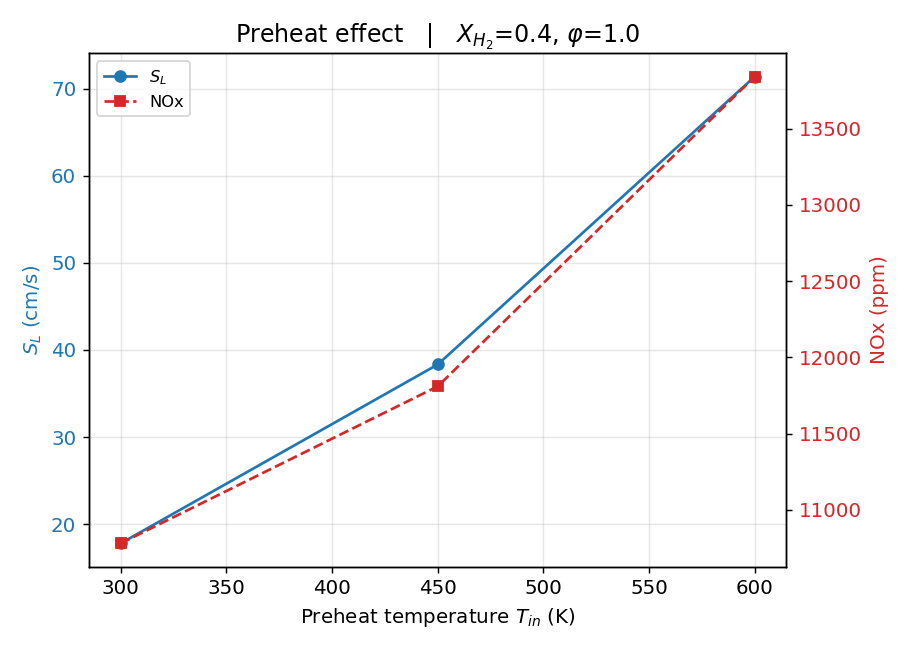
\includegraphics[width=0.80\textwidth]{fig5_preheat.png}
  \caption{Effect of preheat temperature on laminar flame speed and exhaust
  \NOx{} ($X_{\HH}=0.4$, $\phieq=1.0$, $p=\SI{1}{\atm}$).}
  \label{fig:preheat}
\end{figure}

% ============ 5. CONCLUSIONS ============
\section{Conclusions}

A parametric Cantera study of one-dimensional laminar \NHH{}/\HH{}/air flames was
carried out, covering hydrogen fractions of $0$--$0.6$, equivalence ratios of
$0.7$--$1.3$ and preheat temperatures of $300$--$\SI{600}{\kelvin}$. The main
findings are:

\begin{enumerate}
  \item \textbf{Hydrogen enrichment strongly accelerates the flame.} At
  stoichiometric, atmospheric conditions the laminar flame speed rises from
  \SI{5.9}{\centi\meter\per\second} (pure ammonia) to
  \SI{48.3}{\centi\meter\per\second} at $X_{\HH}=0.6$ --- about an eight-fold
  increase. The peak flame speed occurs near $\phieq=1.1$ for every blend.

  \item \textbf{\NOx{} peaks lean and collapses rich.} The highest \NOx{} occurs
  at $\phieq\approx0.8$--$0.9$, while fuel-rich operation reduces \NOx{} by up to
  an order of magnitude through \NO{} consumption by amine radicals.

  \item \textbf{The best compromise is mildly rich operation.} The Pareto front
  of the flame-speed / \NOx{} trade-off is dominated by points at
  $\phieq\approx1.2$--$1.3$, which keep most of the hydrogen-enrichment benefit
  while strongly cutting \NOx{}.

  \item \textbf{Preheating is an efficient lever.} Raising $T_\mathrm{in}$ from
  $300$ to \SI{600}{\kelvin} quadruples \SL{} at only a moderate \NOx{} penalty.
\end{enumerate}

The principal limitation is the use of GRI-Mech~3.0, which was optimised for
natural-gas rather than ammonia chemistry; the absolute \NOx{} levels reported
here should be treated as indicative. A natural extension is to repeat the study
with a dedicated \NHH{}/\HH{} mechanism (e.g.\ Okafor or Stagni) and to compare
the two, and to add a final high-fidelity run with multicomponent transport for
the recommended operating points.

% ============ REFERENCES ============
\begin{thebibliography}{9}
\bibitem{cantera} D.~G.~Goodwin et al., \emph{Cantera: An Object-oriented
Software Toolkit for Chemical Kinetics, Thermodynamics, and Transport
Processes}, version 3.2, 2025. \url{https://www.cantera.org}
\bibitem{gri30} G.~P.~Smith et al., \emph{GRI-Mech 3.0}.
\url{http://combustion.berkeley.edu/gri-mech/}
\bibitem{kobayashi} H.~Kobayashi, A.~Hayakawa, K.~D.~K.~A.~Somarathne,
E.~C.~Okafor, \emph{Science and technology of ammonia combustion},
Proceedings of the Combustion Institute, 37(1):109--133, 2019.
\bibitem{law} C.~K.~Law, \emph{Combustion Physics}, Cambridge University Press,
2006.
\end{thebibliography}

\end{document}
